\documentclass[12pt, a4paper]{article}
\usepackage{polyglossia}
\usepackage{geometry}
\usepackage{lua-ul}
\usepackage{hyperref}
\usepackage{graphicx}
\usepackage{enumitem}
\usepackage{color,soul}

\setlength\parindent{0pt}

\setmainfont{EB Garamond}
\newfontfamily\fonthead{AlegreyaSansSC}
\newfontfamily\fontsub{Bely}

%sections
\newcommand{\head}[1]{
  \phantomsection
  \section*{\centering{\fonthead{#1}}}
  \addcontentsline{toc}{section}{#1}
}

\newcommand{\subhead}[1]{
  \phantomsection
  \subsection*{\centering{\fontsub{#1}}}\vspace{1em}
  \addcontentsline{toc}{subsection}{#1}
}


\newcommand{\subheadfoot}[2]{
  \phantomsection
  \subsection*{\texorpdfstring{\centering\fontsub{#1\protect\footnote{#2}}}{#1}}\vspace{1em}
  \addcontentsline{toc}{subsection}{#1}
}

\newcommand{\subheadfootb}[2]{
  \phantomsection
  \subsection*{\texorpdfstring{\fontsub{#1\protect\footnote{#2}}}{#1}}\vspace{1em}
  \addcontentsline{toc}{subsection}{#1}
}


\newcommand{\subsubhead}[1]{
  \phantomsection
  \subsubsection*{\fontsub{#1}}
  \addcontentsline{toc}{subsubsection}{#1}
}


\newcommand{\subsubheadfoot}[2]{
  \phantomsection
  \subsubsection*{\texorpdfstring{\fontsub{#1\protect\footnote{#2}}}{#1}}
  \addcontentsline{toc}{subsubsection}{#1}
}

\newcounter{quotenum}


\newcommand{\quotehead}[1]{
  \stepcounter{quotenum}
  \phantomsection
  \subsubsection*{\texorpdfstring{\fontsub{\textit{#1}}}}
  \addcontentsline{toc}{subsubsection}{
  Quote \arabic{quotenum}}
}


\newcommand{\titlehead}[2]{
\begin{center}
{\fonthead
\textbf{\huge{#1}}\\[0.1in]
\LARGE{#2}\\[0.2in]
}
\end{center}
}

\newcommand{\ind}{\hspace{1.5em}}


\begin{document}

\newgeometry{top=0.4in,bottom=0.8in}

{\small{\textcolor{red}{*For first and second exam read: page 1,2,3, quotes, short questions and 
characters.}}}


\titlehead{Emma}{Jane Austen}


\subhead{Overview \& Plot}

\ind \textit{Emma}, written in \underLine{1815}, is a \underLine{comedy of manners} 
set in \underLine{Highbury} about Emma's 
struggle with blindness and her fear of confronting her own feelings which leads
her to meddle harmfully in the lives of others. The novel uses free indirect discourse
where the narrator\footnote{\, an anonymous who tells the reader how characters feel and think,
and who also provides insight and commentary.}
steps in and out of Emma’s thoughts. It is narrated in the third person and 
the immediate past tense. It sometimes uses flashbacks, to provide information about
earlier events, and foreshadowing, to provide hints about the future. The below 
diagram shows the structure of the plot:


\begin{figure}[ht]
  \centering
  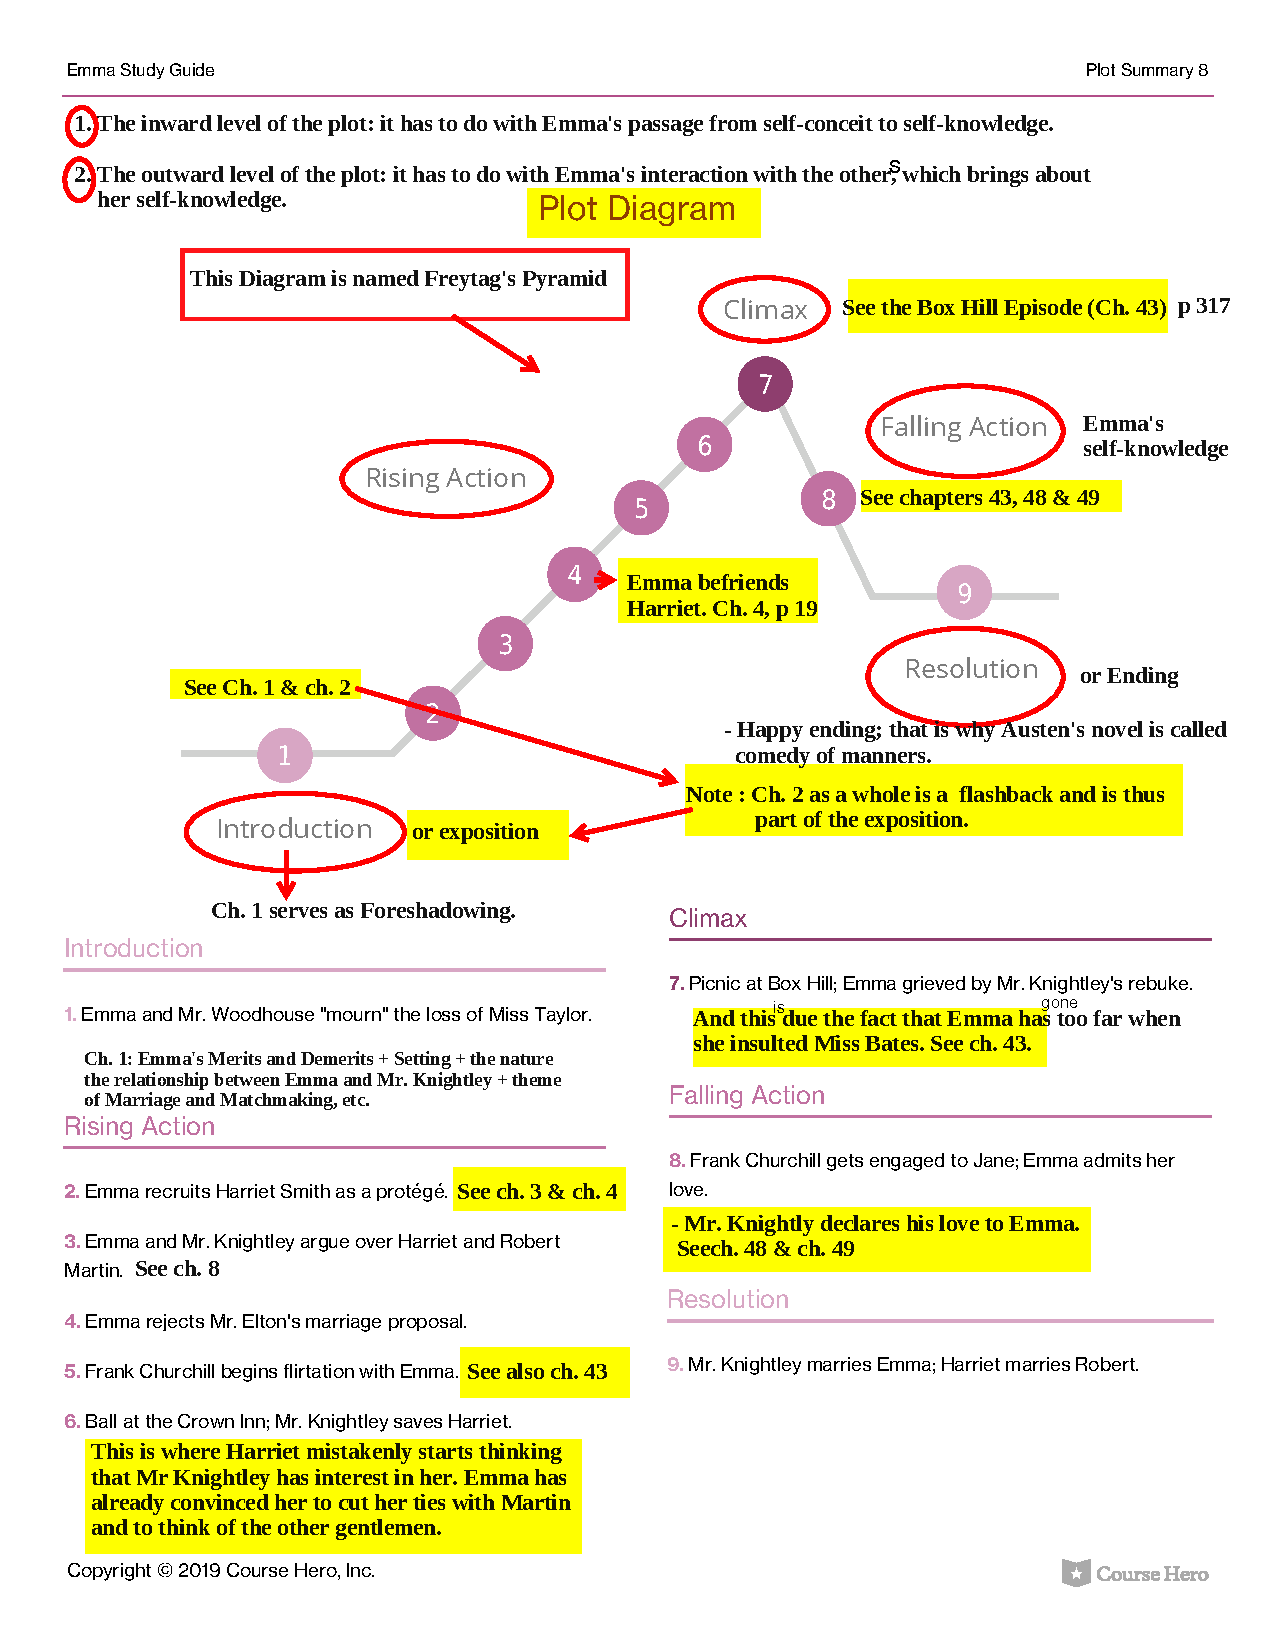
\includegraphics[width=0.9\textwidth]{diagram.pdf}
\end{figure}

\newpage
\subhead{Characters \& Techniques}

\subsubhead{Foreshadowing} 

A narrative technique where a writer hints at events 
that will occur later in the story. Almost every chapter includes 
a foreshadowing, below are some examples:\medbreak

Example from Chapter 1: “The real evils indeed, of Emma’s situation were the power of 
having rather too much her own way, and a disposition to think 
a little too well of herself.”\medbreak

Example from Chapter 27: “felt as if the spring would not pass without bringing a crisis,
an event, a something to alter her present composed and tranquil state.”

\subsubhead{Flashback}

Is when the linear sequence of narration is 
cut and it goes back to the past events. A good example is the story 
of Mr. Weston's first marriage in Chapter 2.



\begin{figure}[ht]
  \centering
  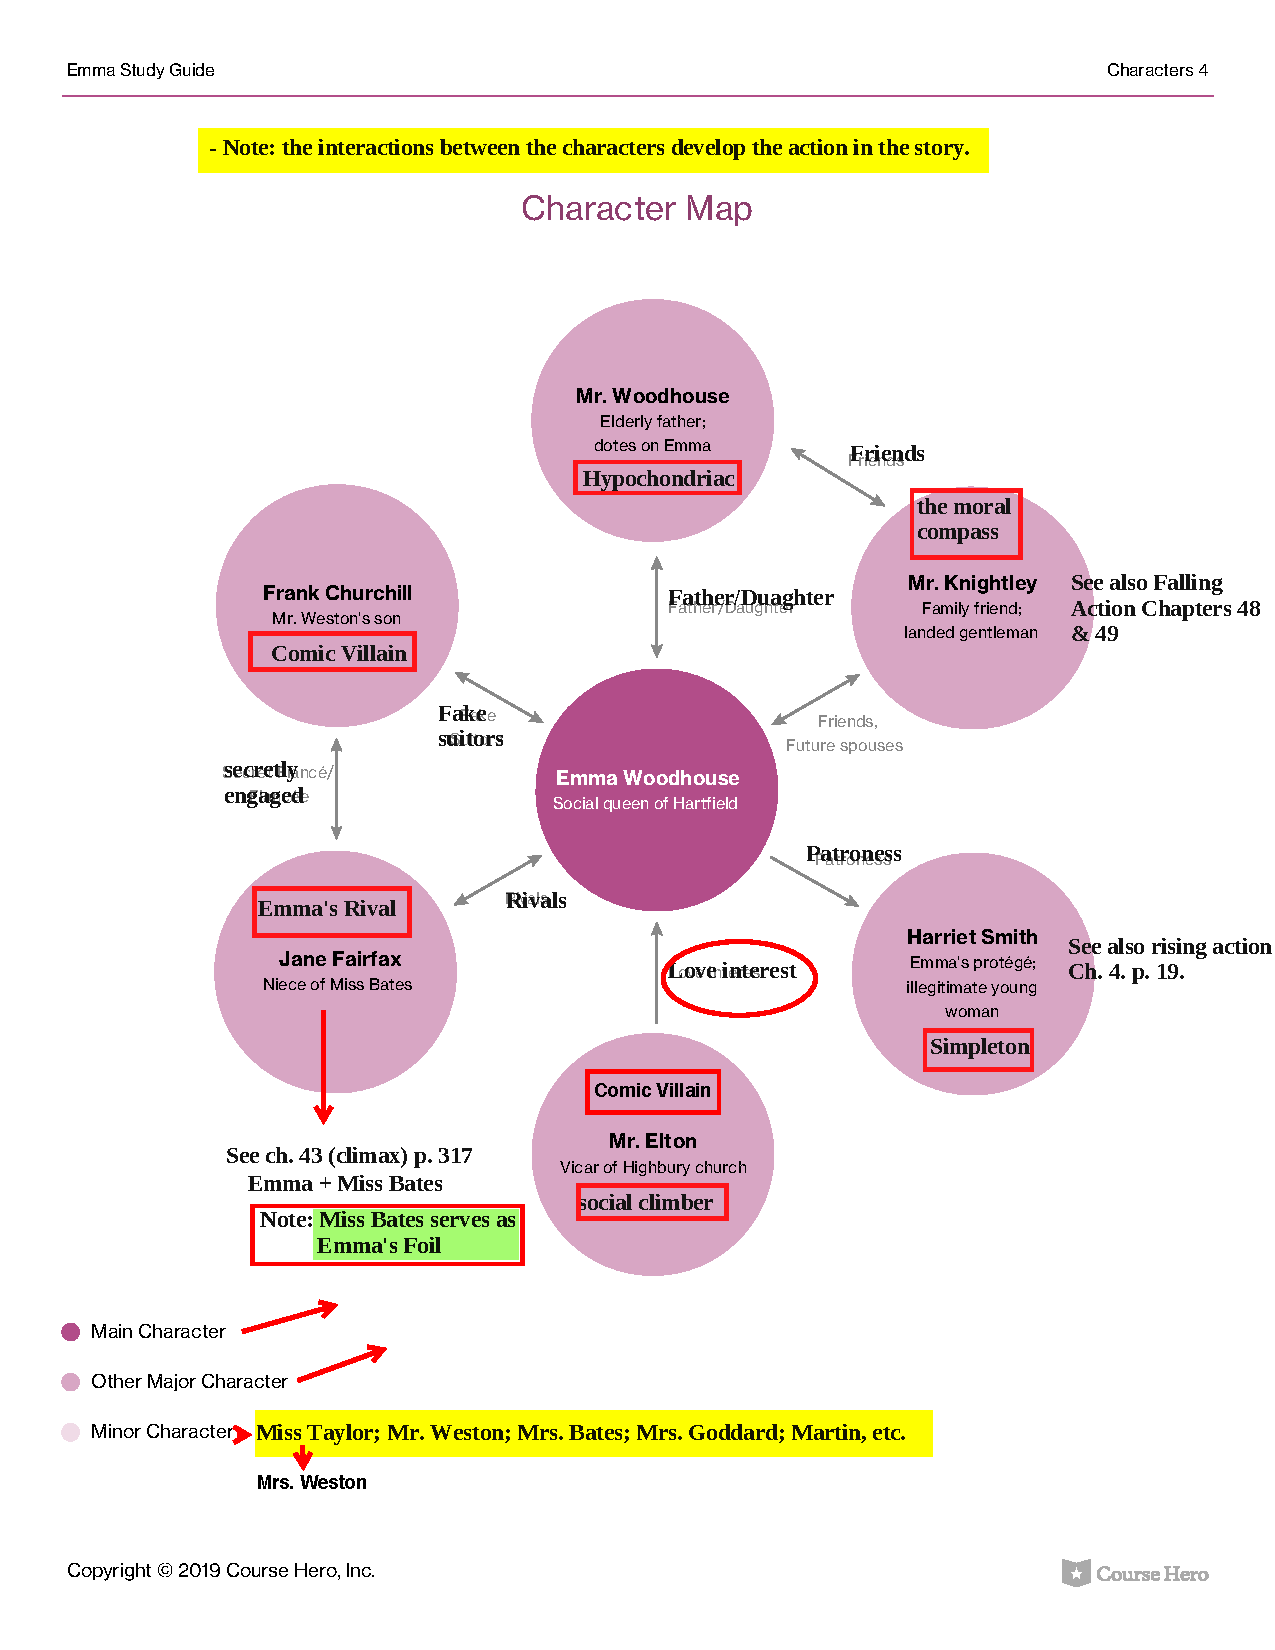
\includegraphics[width=0.9\textwidth]{characters.pdf}
\end{figure}

\restoregeometry




\subhead{Plot Diagram}

\subsubhead{Exposition}

\ind Or the introduction, is the part of the story where we are given an idea about some of the major 
characters, themes and settings. In \textit{Emma}, the exposition includes both chapter 1 and 2. In
the exposition we are told about Emma merits and demerits, we are also introduced to the main
characters and Emma's relationship with them.


\subsubhead{Rising Action}

\ind The part of the story where the conflict begins and the main character 
seeks to overcome their struggles. In \textit{Emma}, the rising action starts after
chapter 2, beginning when Emma takes Harriet under her wing.
At this point, Emma begins to project her own feelings and desires onto Harriet. 
Convinced that Mr. Elton 
is a better match for Harriet, Emma convinces her to refuse Robert Martin’s proposal.
This marks the start of the rising action.

\subsubhead{Climax}

\ind The part of the story of the most intense moment, marking the turning point of the main
character. In \textit{Emma} we see this in Chapter 43, when Emma insults Miss Bates in the Box 
Hill picnic, and then she is scolded by Mr. Knightley. She realizes she is in love with him after 
being jealous of Harriet’s feelings for Mr. Knightley. 

\subsubhead{Falling Action}

\ind The part of the story that follows the climax, clarifies the narrative,
and leads toward the resolution. In \textit{Emma}, the resolution happens when Emma 
and Mr. Knightley confess their feelings for one another, and Mr. Knightley proposes to
Emma. Harriet accepts Mr. Martin’s proposal and Jane and Frank prepare to marry.

\enlargethispage{\baselineskip}
\subhead{Estates}\vspace{-3mm}

\begin{itemize}
  
\item \textbf{Hartfield}, where Mr. Woodhouse (Henry) and Emma live.

\item \textbf{Randalls}, where the Westons live.

\item \textbf{Enscombe}, where the Churchills live.

\item \textbf{Donwell Abbey}, where Mr. George Knightley live.

\item \textbf{Abbey-Mill Farm}, where the Martins live, it is part of Downwell Abbey.
  
\item \textbf{Brunswick Square}, where Mr. John Knightley and Isabella\footnote{\, Emma's sister.} live.

\end{itemize}


\subhead{Forms Of Irony}

\subsubhead{Situational Irony}

When the outcome of an event is the opposite of what the character expect.
A good example is when Emma discourages Harriet
from accepting Robert Martin's proposal because she thinks he is not fit for her.
However, in the end it is revealed that Mr. Martin is the best match for Harriet.

\subsubhead{Dramatic Irony}

When the reader knows something that the character does not know. A good example is
when Emma thinks that Mr. Elton is a good match to Harriet, while the reader knows
that Mr. Martins is the better match. 

\subsubhead{Verbal Irony}

Or sarcasm, is saying the opposite of what you mean. A good example is when 
Mr. Knightley says,"A worthy employment for a young lady's mind!" during 
his conversation with Emma about matchmaking. What he really means is that
she is wasting her merits on matchmaking.


\subhead{Draw a Character Sketch of the Following}

\subsubhead{Emma Woodhouse}

Handsome, clever, rich, and somewhat spoiled. She is twenty one when the story opens.
Her mother died when she was five, after that Miss Taylor became her governess.
She has been mistress of the house since her older sister got married. Although smart, 
she lacks the discipline to practise or study anything in depth. She is
portrayed as compassionate to the poor, but at the same time has a
strong sense of class status (\hl{snobbish}). Being spoiled and vain makes her \hl{blind} to 
her feelings and the feelings of others, and she ends up hurting both. She suffers from 
\hl{intellectual solitude} after Miss Taylor marries Mr. Weston.

\subsubhead{Mr. George Knightley}

George Knightley is a gentleman and a longtime family friend of the Woodhouse family.
He is considerate, aware of the feelings of the other characters, and 
always exhibits good behaviour and judgment.
He is the \hl{moral compass} of the story and Emma's only critic. He owns Donwell Abbey where the Martins
have a farm. He is thirty-seven when the story opens and the elder brother 
of Mr. John Knightley, the husband of Emma's elder sister Isabella.

\subsubhead{Harriet Smith}

Beautiful, naive, and fair, with a fine bloom, blue eyes, light hair,
regular feature, and a look of great sweetness. She was seventeen when the story opens.
She is the illegitimate daughter of somebody. She lived with Mrs. Goddard, who introduce her
to Emma. Emma
becomes her friend and takes her under her wing. However, she turns out to be a bad influence
on Harriet because she projects her own desires and beliefs onto her. Harriet is described as 
a \hl{simpleton} by Mr. Knightley because she refuses Robert Martin's proposal.

\subsubhead{Mr. Elton}

Good-looking, well-mannered, and ambitious. Twenty seven years old and unmarried when the story opens.
He gets his living by being the \hl{vicar} of Highbury and he lives alone in the vicarage where he suffers
from \hl{blank solitude}. He is a \hl{social climber}, he wants to marry a wealthy woman so he go up 
the social ladder. After Emma
rejects him, he soon marries Miss Hawkins, proving he never truly cared for Emma.

\subsubhead{Mr. Henry Woodhouse}

Is the father of Emma and the owner of Hartfiled. He is generous and well mannered,
although his fastidious nature and his hate for change
make it a somewhat difficult for others to get along with him. He enjoys keeping a small circle of 
people around him and only invites them to his own house on his own terms. He is the reason Emma does not consider marriage, 
because marriage is the origin of change. Despite being self-centered and unable to see beyond his own feelings,
he is kind and well-respected by others. He is associated with the term \hl{gentle selfishness} and
\hl{fastidious}, \hl{valetudinarian} or \hl{hypochondriac}\footnote{\, all three have the same meaning; a person that is 
very concerned about his health and hateful of the idea of change.}.

\subsubhead{Miss Bates}

Is an old, alright looking, poor spinster who lived with her mother 
and spent most of her youth caring for her. She was simple 
and cheerful which made her popular in Highbury. She loved everybody and was 
interested in everybody's happiness. She was full of trivial communications
and harmless gossip. She is considered to be \hl{Emma's foil} because she lack all the
merits Emma has.

\enlargethispage{\baselineskip}

\subsubhead{Mr. Weston}

Is a kind and cheerful man who enjoys people’s company, and was a native of Highbury.
After joining the militia he marries Miss Churchill and they have a son named Frank,
soon after Miss Churchill dies and due to financial struggles Mr. Weston, decided
to give Frank to the Churchills family to take care of him. Later, after establishing 
himself in trade and marrying Miss Taylor, he moved with her to live at Randalls.

\subsubhead{Frank Churchill}

Is handsome, charming, and witty. He is Mr Weston's son by his first marriage but 
was raised by his wealthy aunt and uncle, the Churchills, at the family estate of Enscombe 
in Yorkshire. He is revealed over the course
of the novel to be a scheming, insincere, and somewhat cowardly man. 
He manipulates and plays games with the other characters to ensure his secret engagement 
to Jane remains concealed that is why he is considered to be a \hl{comic villain}.

\subsubhead{Jane Fairfax}

Is an orphan whose only family is her aunt, Miss Bates, and her grandmother, Mrs Bates.
Though a native of Highbury, she was educated and nurtured by the
Campbells, who had been friends of her father. She is a beautiful, bright, and elegant woman
but because of her unpleasant situation, she is destined to be a governess. She is secretly 
engaged to Frank Churchill. She is considered as \hl{Emma’s rival} though she is far more accomplished,
which makes Emma envy her.




\subheadfoot{Emma Major Motifs}{\, a motif is a recurring symbol, idea, or image that appears across a story to develop
its major themes.}


\subsubhead{Bad Parenting}

\ind In \textit{Emma}, we see few characters being bad parents to their children:
The first is Mr. Woodhouse (Henry), his fastidious nature and hatred of change prevent 
Emma from even considering marriage. The second is Weston, after facing financial struggles, 
he abandons his son Frank, leaving him in the care of his late wife’s relatives (the Churchills)
The third is Harriet's parents, they abandon her in childhood leaving her in the custody of
Mrs. Goddard’s.



\subsubheadfoot{Blindness}{\, similar to the theme of the blinding power of imagination.}

\ind In \textit{Emma} , few characters show blindness to the truth because of their biases and desires.
We see it in Emma when she misunderstands the motives of Mr. Elton, thinking  
that he is in love with Harriet while he actually has feelings for Emma. Her desire
to match Mr. Elton with Harriet blinds her to his true feelings. Similarly,
when she speaks cruelly of Jane Fairfax, it stems from her jealousy of Jane’s accomplishments. We also see
this blindness in Mr. Knightley; he criticizes Frank Churchill not on the basis of truth, but rather 
out of jealousy because of Frank's relationship with Emma.

\subsubhead{Visits}

\ind The main events of the novel take place during visits that the characters pay to each other. The
frequency and length of visits between characters indicates the level of intimacy and attachment
between them. Frank’s frequent visits to Hartfield show his relationship with Emma to be close.
Mr. Knightley’s constant presence at Hartfield indicates his affection and regard for Emma.
Emma encourages Harriet to limit a visit with the Martin family to fifteen minutes, because such a
short visit clearly indicates that any former interest has been lost. 

\subsubhead{Parties}

\ind In \textit{Emma} , parties center on social conventions more than around
individual attachments. Emma’s hosting a dinner party for Mrs. Elton, a woman she dislikes,
exemplifies this characteristic. There are six important parties in the novel: the Christmas Eve party at
Randalls, the dinner party at the Coles’, the dinner party given for Mrs. Elton, the dance at the Crown
Inn, the morning party at Donwell Abbey, and the picnic at Box Hill. Each occasion provides characters 
with opportunities to observe one another and witness social interactions.


\subheadfoot{Emma Major Symbols}{
\, symbols are objects, characters, figures, or colors used to represent abstract ideas or concepts.}

\subsubhead{The Word Game}

\ind A word game is played in Chapter 41 between Emma, Frank, and Jane. It functions
as a metaphor for the partial understandings and misunderstandings that exist among Emma, Frank,
Jane, and Mr. Knightley. As Mr. Knightley looks on, Frank uses child’s blocks to create words for the
ladies to decode, though these words mean different things to each of them. Frank makes the word
“blunder,” which Jane understands as referring to a mistake he has just made, but whose meaning is
opaque to Emma and Knightley. He then makes the word “Dixon,” which Emma understands as a joke
on Jane, and which baffles Knightley. In truth, everyone “blunders” in different ways that evening,
because no one possesses complete enough information to interpret correctly everything that is going
on.


\subsubhead{The Riddle}

\ind Also known as charades, riddles in the novel take the form of elaborate wordplay. They symbolize the
pervasive subtexts that wait to be decoded in characters’ larger social interactions. In Chapter 9, Mr.
Elton presents a riddle to Emma and Harriet. Emma decodes it immediately, as “courtship,” but she
decodes it wrongly in the sense that she believes it is meant for Harriet rather than herself. This
wordplay also makes an appearance during the Box Hill party, when Mr. Weston makes an acrostic for
Emma.


\subsubhead{Tokens of Affection}

\ind A number of objects in the novel take on symbolic significance as tokens of affection. Mr. Elton frames
Emma’s portrait of Harriet as a symbol of affection for her, though Emma misunderstands it as a symbol
of affection for Harriet. Harriet keeps court plaster and a pencil stub as souvenirs of Mr. Elton. When the
engagement between Jane and Frank is briefly called off, she returns his letters to symbolize her
renunciation of his affection.

\subheadfoot{Emma Major Themes}{\, themes are the fundamental ideas explored in a literary work.}

\subsubhead{Marriage and Social Status}

\ind \textit{Emma} is structured around marriage, which was one of the
main ways to raise one’s social status, especially for women, 
who were denied the possibility of improving their status through hard
work or personal achievement. In Austen’s time, social status was
determined by a combination of family background, reputation, and wealth-marriage.
Yet, the novel suggests that marrying too far above oneself leads to strife.
This is shown in the marriage of Mr. Weston to Miss Churchill where the inequality 
of the relationship causes hardship to both. Another example is Emma’s attempt to match Harriet with
Mr. Elton who shows disinterest in Harriet because she is a foundling daughter of nobody.
The novel present equal marriage as ideal, which is shown in the marriage of Emma to Mr. Knightley
and Harriet to Robert Martin.

\subsubhead{The Confined Nature of Women’s Existence}

\ind The novel gives a strong sense of the confined nature of a woman’s existence in 
early-nineteenth-century rural England. Emma possesses a great deal of intelligence and 
energy, but the best use she can make of these is matchmaking, something that 
gets her into trouble. The alternative pastimes shown in
the novel such as social visits, charity visits, music, artistic endeavors seem relatively trivial.
There were not many options for women back then: they could become governesses or marry.
If, however, a woman was fortunate enough to be financially independent, she could remain a spinster. 
Marriage offered women power and affect over their own destinies. 
Participating in the rituals of courtship and accepting or
rejecting proposals is perhaps the most active role that women are permitted to play in Emma’s world.

\newpage
\subsubheadfoot{The Blinding Power of Imagination}{\, similar to the motif of blindness.}

\ind The novel illustrates the ways in which personal biases and desires blind
objective judgment. Emma’s desire to match Harriet to Mr. Elton blinds her to the
fact that Mr. Elton had feelings for her all along. Mr. Knightley's judgment of Frank Churchill 
is biased because he is jealous of Frank’s relationship with Emma, and Emma speaks cruelly of
Jane because her vanity makes her jealous of Jane’s accomplishments. Emma’s biases cause her to
invent an attachment between Harriet and Frank and blind her to the fact that Harriet actually has
feelings for Knightley. The detachment of the narrator allows us to see many of these
misunderstandings before the characters do. And the plot is powered by a series of realizations 
that permit each character to make fuller, more objective judgments.

\subsubhead{The Obstacles to Open Expression}

\ind The misunderstandings happening  in the novel are created, in part, by the conventions of
social decency. As a result characters are unable to express their feelings directly and openly,
and their feelings are therefore mistaken. In the novel we see two ways of expression:
the first is the natural, warm, and direct manner of both Mr. Knightley and
Mr. Martin; The second is the overly clever and complex speech of 
Mr. Elton, Frank Churchill, and Emma. Austen seems to prefer the first kind while condemning 
the second as misleading and deserving censure. We see the second kind when Emma cruelly insults Miss Bates.
The novel by no means suggests that the manners and rituals of social interaction should be eliminated,
but rather handling them with tactful tacitness.



\subhead{Emma: Important Quotes}\vspace{-3mm}


\quotehead{
"Emma Woodhouse, handsome,
clever, and rich, with a comfortable
home and happy disposition,
seemed to unite the best
blessings of existence; and had
lived nearly twenty one years in
the world with very little to
distress or vex her." 
}

\, — Chapter 1, Exposition \medbreak

These words are said by the narrator in the exposition about the hero of the novel, Emma.
She is described as having the best that life can offer. However, the narrator uses an ironic tone
which makes us wonder; is Emma going to make use of her merits? 

\enlargethispage{\baselineskip}

\quotehead{
"And have you never known the pleasures and triumph of 
a lucky guess? I pity you."
}

\, — Chapter 1, Exposition \medbreak

These words are said by Emma during a conversation with Mr. Knightley about matchmaking.
Emma believes she is the reason why Miss Taylor and Mr. Weston were married, while Mr. Knightley 
tells her it was merely a matter of guessing.

\quotehead{
"The real evils, indeed, of Emma’s situation were the power of having rather too much her
own way, and a disposition to think a little too well of herself: these were the disadvantages
which threatened alloy to her many enjoyments. The danger, however, was at present so
unperceived, that they did not by any means rank as misfortunes with her."
}


\, — Chapter 1, Exposition \medbreak

These words are said by the narrator in the exposition about Emma's demerits. The narrator foreshadows the novel’s
structure as a whole: Emma having too much of her way and her vanity makes her blind to her
feelings and the feelings of others. This causes her to meddle in the life of others, harming both them and herself.


\quotehead{
“Of this great intimacy between Emma and Harriet Smith , but I think it a bad thing“
}

\, — Chapter 5, Rising Action\medbreak

These words are said by Mr. Knightley to Mrs. Weston about Emma and Harriet relationship.
He explains that Emma is a bad influence on Harriet, projecting her own desires and needs
onto Harriet and making her think that she is the daughter of a gentleman.



\quotehead{
“She always declares she will never marry which of course, means just no thing at all “ 
}

\, — Chapter 5, Rising Action\medbreak

These words are said by Mrs. Weston to Mr. Knightley when they were talking about Emma. 
She says that Emma's refusal of marriage is not serious, and eventually she
will find someone whom she could love and marry.

\quotehead{
“This man is almost too gallant to be in love“
}

\, — Chapter 5, Rising Action\medbreak

These words are said by Emma to herself about Mr. Elton. She thinks that
Mr. Elton is not genuine about his feelings for Harriet. However, she dismisses
this doubt because of her high confidence as a match-maker, which blinds her to
the fact that she is wrong in her judgement about other people.

\quotehead{
“Not Harriet equal!! No he is not her equal he is as much her superior in sense as in situation“
}


\, — Chapter 8, Rising Action\medbreak

These words are said by Mr. Knightley to Emma after she tells him that Robert Martin is not Harriet's
equal because he is a farmer while she is supposedly a gentleman's daughter. Mr. Knightley counters
that Harriet is a foundling girl with no family background, and that Martin is better suited than her in
both social standing and intelligence.


\quotehead{
“Upon my word Emma to hear you abusing the reason you have, is almost enough to make me think so too, 
better be without sense than misapply it as you do.“
}


\, — Chapter 8, Rising Action\medbreak

These words are said by Mr. Knightley to Emma after she claims that Harriet's
beauty entitles her to pick and choose between men, and that Robert Martin is inferior to her
in rank. Knowing Emma to be intelligent, Mr. Knightley reflects that lacking reason would be 
better than having it and misusing it.


\quotehead{
"Then she is greater simpleton than i ever believed her, what is the foolish girl about?"
}

\, — Chapter 8, Rising Action\medbreak


These words are said by Mr. Knightley to Emma about Harriet after Emma tells him that she 
refused Robert Martin's proposal. He is enraged by this because he thinks that
Robert is a good match for Harriet.


\quotehead{
"Harriet Smith may not find offers of marriage flow in so
fast, though she is a very pretty girl. Men of sense, whatever 
you may choose to say, do not want silly wives. Men of 
family would not be very fond of connecting themselves with a girl 
of such obscurity—and most prudent men would
be afraid of the inconvenience and disgrace they might be
involved in, When the mystery of her parentage came to be reveled."
}

\, — Chapter 8, Rising Action\medbreak

These words are said by Mr. Knightley to Emma after she tells him that Harriet's beauty gives 
her the power to choose. Mr. Knightley tells her that because Harriet is a foundling girl, men
would not want to associate with her.

\quotehead{
“But then to be an old maid at last, like Miss Bates!"\\
"That is as formidable an image as you could present,
Harriet; and if I though I should ever be like Miss Bates—so silly, so satisfied, so smiling
so prosing, so undistinguishing and unfastidious, and so apt 
to tell everything relative to everybody about me, I would marry to-morrow."
}

\, — Chapter 10, Rising Action\medbreak

These words are said by Emma when Harriet compares her to Miss Bates. Emma tells her
that she is nothing like Miss Bates, saying that Miss Bates is chatty and naive. This reveals
Emma's snobbery and her strong sense of class status.


\newpage
\quotehead{
“Never mind, Harriet, I shall not be a poor old maid and it is
poverty only which makes celibacy contemptible to a generous
public! A single woman with a very narrow income must be a
ridiculous, disagreeable old maid! the proper sport of boys and girls 
but a single woman of good fortune is always respectable,"
}

\, — Chapter 10, Rising Action\medbreak

These words are said by Emma during a conversation with Harriet about Miss Bates. Harriet triggers 
Emma's fears about the future by suggesting that she will become just like Miss Bates--old and single. 
However, Emma rationalizes this fear by arguing that only poverty that makes celibacy undesirable.



\quotehead{
“Ah! ma’am, but there may be a difficulty. Pardon me, but you will be limited as to
number—\- only three at once.”
}

\, — Chapter 43, Climax\medbreak

These words are said by Emma to Miss Bates during the Box Hill picnic. Emma tells 
Miss Bates that she is capable of coming up with more than plenty of dull ideas and 
comments, and that it would be best to limit her before she starts – Insulting her
in front of everyone. 

\quotehead{
"How could you be so unfeeling to Miss Bates? How could you be so insolent to a woman of her character, 
age, and situation ? Emma i had not though it possible."
}


\, — Chapter 43, Climax \medbreak

These words are said by Mr. Knightley to Emma after she insulted Miss Bates in the Box Hill picnic.
He scolds Emma for being rude to Miss Bates and embarrassing her in front of everyone, reminding 
her that she should sympathize with Miss Bates because of her unfortunate situation.

\quotehead{
"She was vexed beyond what could have been expressed—almost beyond what she could
conceal. Never had she felt so agitated, so mortified, grieved, at any circumstance in her life.
She was most forcibly struck. The truth of his representation there was no denying. She felt it
at her heart. How could she have been so brutal, so cruel to Miss Bates! How could she have
exposed herself to such ill opinion in any one she valued! And how suffer him to leave her
without saying one word of gratitude, of concurrence, of common kindness!"
}


\, — Chapter 43, Climax\medbreak

These words are said by the narrator about Emma after Mr. Knightley scolds her for
insulating Miss Bates at the Box Hill picnic. As she realize the cruelty of her action,
she experiences intense remorse. This mark the point where Emma grow and understand 
how wrongly she has treated Miss Bates. This moment is also Emma’s most emotional in the novel.


\newpage
\quotehead{
"She is poor; she has sunk from
the comforts she was born to; and,
if she live to old age, must
probably sink more. Her situation
should secure your compassion. It
was badly done, indeed!"
}

\, — Chapter 43, Climax\medbreak

These words are said by Mr. Knightley to Emma after she insults Miss Bates in front of everyone
in the Box Hill picnic. Mr. Knightley scolds her for lack of feeling, and shows himself to be
the moral compass of the story and the judge of Emma's actions.


\quotehead{
"I assure you she did. She felt your full meaning. She has
talked of it since. I wish you could have heard how she talked of it"
}

\, — Chapter 43, Climax \medbreak

These words are said by Mr. Knightley to Emma after she insulted Miss Bates in the Box Hill picnic. Emma thinks that
Miss Bates is not smart enough to understand her insult, but Mr. Knightley assures her that
Miss Bates did.




\enlargethispage{\baselineskip}
\quotehead{
"Emma’s eyes were instantly withdrawn; and she sat silently meditating, in a fixed attitude,
for a few minutes. A few minutes were sufficient for making her acquainted with her own
heart. A mind like hers, once opening to suspicion, made rapid progress; she touched, she
admitted, she acknowledged the whole truth. Why was it so much worse that Harriet should
be in love with Mr. Knightley than with Frank Churchill? Why was the evil so dreadfully
increased by Harriet’s having some hope of a return? It darted through her with the speed of
an arrow that Mr. Knightley must marry no one but herself!"
}

\, — Chapter 47, Falling Action\medbreak

These words are said by the narrator about Emma when she was having a conversation with Harriet,
in which Harriet confesses her feelings for Mr. Knightley. Emma's jealousy of Harriet makes her
realize that she is in love with Mr. Knightley. For the majority of the novel she is blind 
because her attention was misdirected towards matchmaking.

\quotehead{
"Seldom, very seldom, does
complete truth belong to any
human disclosure; seldom can it
happen that something is not a
little disguised, or a little mistaken;
but where, as in this case, though
the conduct be mistaken, the
feelings are not, it may not be very
material."
}


\, — Chapter 47, Falling Action\medbreak

These words are said by the narrator in chapter 49 after Mr. Knightley and Emma betrothal.
The quotation explains that it is often difficult to tell the whole, literal truth, and at
times to do so would actually hinder human relations. In such
instances the ends may justify the means.

\newpage
\quotehead{
"Marriage, in fact, would not do for her. It would be
incompatible with what she owed to her father, and
with what she felt for him. Nothing should separate her from her father.
She would not marry, even if she were asked by Mr Knightley."
}

\, — Chapter 48, Falling Action\medbreak

These words are said by the narrator about Emma's thoughts after she realizes her feelings for Mr. Knightley.
Because of her attachment to her father, Emma tries to push away any thoughts of marriage, even to Mr. Knightley.


\quotehead{
"I have never had a high opinion of Frank Churchill. I can
suppose, however, that I may have underrated him. 
—My acquaintance with him has been but trifling. 
And even if have
not underrated him hitherto, he may yet turn out well.
With such a woman he has a chance. I have no motive for wishing
him ill—and for her sake, whose happiness will be involved in his good character and conduct, I shall certainly wish him
well.”
}

\, — Chapter 49, Falling Action\medbreak

These words are said by Mr. Knightley to Emma about the relationship between 
Jane Fairfax and Frank Churchill. He admits that he may have misjudged Frank and 
expresses how lucky Frank is to be engaged to a woman like Jane.

\quotehead{
“If I loved you less, I might be able to talk
about it more. But you know what I am. You hear nothing but
truth from me. I have blamed you, and lectured you, and you 
have borne it as no other woman  in England would have 
borne it. Bear with the truths I would tell you now, dearest Emma,
as well as you borne with them. The manner, perhaps, may
have as little to recommend them.
}

\, — Chapter 49, Falling Action\medbreak

These words are said by Mr. Knightley to Emma during his declaration of love.
He tells her that she has endured his scolding and blame as no other woman would have.
This is the most critical moment in the novel.

\enlargethispage{\baselineskip}
\subheadfoot{Less Important Quotes}{\, these quotes are seen in the \textbf{Abridged Notes}
and are less likely to be in the first and second exam, they only matter in the final exam.}

\setcounter{quotenum}{0}

\quotehead{
"A young farmer ... is the very last
sort of person to raise my
curiosity. The yeomanry are
precisely the order of people with
whom I feel I can have nothing to
do."
}

\, — Chapter 3, Rising Action\medbreak

These words are said by Emma about Robert Martin when she was talking with Harriet.
She reveals a shocking degree of snobbery in her desire to distance herself from Martin.
As a result, she tries to make Harriet lose interest in Martin.


\quotehead{
"I confess that I have seldom seen
a face or figure more pleasing to
me that hers. But I am a partial old
friend."
}

\, — Chapter 5, Rising Action\medbreak

These words are said by Mr. Knightley about Emma when he was talking to Mrs. Weston.
She pushes him to acknowledge Emma's physical beauty, but he hardly wants to
admit his attraction, undercutting his statement by saying he may be partial because he is an old friend.

\quotehead{
"Till it appears that men are much
more philosophic on the subject of
beauty than they are generally
supposed; till they do fall in love
with well-informed minds instead
of handsome faces, a girl, with
such loveliness as Harriet, has a
certainty of being admired and
sought after, of having the power
of choosing from among many."
}

\, — Chapter 8, Rising Action\medbreak

These words are said by Emma when she was arguing with Mr. Knightley about
whether Martin is a good fit for Harriet. She responds that Harriet's
beauty give her the privilege to choose, and that men only care about
beauty when looking for a wife.

\quotehead{
"The first error, and the worst, lay at her door. It was foolish, it was wrong, to take so active a
part in bringing any two people together. It was adventuring too far, assuming too much,
making light of what ought to be serious—a trick of what ought to be simple. She was quite
concerned and ashamed, and resolved to do such things no more."
}

\, — Chapter 16, Rising Action\medbreak

These words are said by the narrator about Emma's reflections after Mr. Elton proposes to her.
She realize how wrong she was in thinking him attached to Harriet. 
She understands what is wrong with matchmaking: that courtship should
be serious and simple; it should flow naturally between two people.



\quotehead{
"You are very fond of bending little
minds; but where little minds
belong to rich people in authority, I
think they have a knack of swelling
out, till they are quite as
unmanageable as great ones."
}

\, — Chapter 18, Rising Action\medbreak

These words are said by Emma to Mr. Knightley when they were talking about Frank Chur\-chill.
After Knightley criticizes Frank for not fulfilling his duty as a son, Emma defends him saying
that he lives under the influence of his aunt who keeps him away from Highbury. In this dialogue she shows her great
use of wit and metaphor.



\quotehead{
"And no great harm if it does, said
Mr. Woodhouse. 'The sooner every
party breaks up, the better."
}

\, — Chapter 25, Rising Action\medbreak

These words are said by Mr. Woodhouse to Mr. Weston when the latter was trying to persuade him
to allow Emma to stay out late when she attends the Coles' dinner party. Mr. Woodhouse comment
show his self-centeredness and selfishness.

\quotehead{
"She did ... regret the inferiority of
her own playing and singing. She
did most heartily grieve over the
idleness of her childhood—and sat
down and practiced vigorously an
hour and a half."
}

\, — Chapter 27, Rising Action\medbreak

These words are said by the narrator about Emma when she felt jealous
of Jane Fairfax's piano playing. Emma feels inferior and blames herself for her lack
of discipline in cultivating her own talents.

\quotehead{
"Why really, dear Emma, I say that
he is so very much occupied by
the idea of not being in love with
her, that I should not wonder if it
were to end in his being so at last."
}

\, — Chapter 33, Rising Action\medbreak

These words are said by Mrs. Weston to Emma about Mr. Knightley. Mrs. Weston
believes that Mr. Knightley has feelings for Jane Fairfax, even after Mr. Knightley
admits otherwise. This is an example of perverse blindness in the face of facts.




\phantomsection
\section*{\centering{\fontsub{\large Provide short answer for each of the following questions}}}
\addcontentsline{toc}{section}{Provide short answer for each of the following questions}

\subheadfootb{Chapter 1-5}{\, first exam questions.}

\subsubhead{What are Emma's merits?}

Handsome, clever, and rich with a conferable home and happy disposition.

\subsubhead{What are Emma's demerits?}

The power of having too much her own way, and a disposition to think a little too well of herself.

\subsubhead{What is the importance  of the opening lines of the novel \textit{Emma}?}

The opening lines, known as the exposition, introduce the characters, setting, and themes of the novel.

\subsubhead{Who was suffering from intellectual solitude and why?}

Emma, because of the marriage of Miss Taylor.

\subsubhead{Who was described as suffering from blank solitude and Why?}

Elton, because he lived alone without liking it.


\subsubhead{Who are The Martins and why Emma wanted Harriet to cut her relationship with them?}

They are farmers who work at Abbey-Mill Farm. Because Emma considers them a bad 
company to Harriet.

\subsubhead{Why Emma thinks Elton as a suitable future husband to Harriet?}

Because he is a gentleman with a comfortable house and money. He also
does not have parents that can prevent such marriage.

\subsubhead{Why Emma chooses Harriet in particular as her project to marry her up with Elton? }

Because she is naive and ignorant and she has no parents that can object to such marriage.

\subsubhead{Who is "little Frank"? And why he was raised by his mother's family?}

He is the son of Mr. Weston. He was brought up by his mother's family because his father 
was not able to afford to raise him.

\subsubhead{What is the important of visits in \textit{Emma}?}

It offers the chance for other characters to meet and interact with each other.

\subsubhead{Define and exemplify the term foreshadowing.}

Answer on page 2.

\subsubhead{Who else is Emma planning to marry up after she made the match of Miss. Taylor and 
Mr. Weston?}

Mr. Elton to Harriet Smith.

\subsubhead{What is the motif of blindness in Emma?}

One example of Emma's blindness occurs when she  misreads Mr. Elton's motives. 
She believes he is in love with Harriet, while he actually has feelings for Emma herself. 
Her desire to match Mr. Elton with Harriet blinds her to the reality of his feelings.




\subheadfootb{Chapter 5-49}{\, second exam questions}

\subsubhead{Why is Miss Bates considered Emma’s foil?}

Because Miss Bates lacks all the merits that Emma has.

\subsubhead{Which character is considered Emma’s rival, and why?}

Jane Fairfax, because she possesses all of Emma's merits except wealth, and she makes better use of them.

\subsubhead{Which character is described as being "simpleton", and why?}

Harriet, for refusing Robert Martin's proposal.


\subsubhead{Which character does Mr. Knightley feel jealous of, and why?}

Mr. Knightley feels jealous of Frank Churchill. Because of Frank relationship with Emma.

\subsubhead{Define and exemplify the term "falling action" in Emma?}

Answer on page 3

\subsubhead{Given the Box Hill episode, do you think that Emma has made use of her advantages?}

No she does not, her rude remark to Miss Bates reflects her lack of consideration for others and
snobbery.


\end{document}
